\chapter{関連研究}

\section{XAI}

\subsection{概要}
XAIとはexplainable AI(説明可能AI)の略語であり、AIを人間に対して説明可能なものにする、もしくは説明可能なAIを構築する領域である。
本論文はAIの判断根拠として先読みを示す意味でXAIの分野に属する研究であると言える。
ここでの「説明可能性」の語は「人間に理解できる形での説明を与える能力」\cite{oord2016wavenet}と定義され、
「いつ、どのような、どのように」説明を与えるかによってさらに細かく分類される。
「いつ」、つまりどの時点で説明を与えるか、に関しては既存のネットワークに対して新たに説明を加える「事後的」説明と初めから動作の根拠を示せるようにネットワークやシステムを構築する「事前的」説明
に分類できる\cite{oord2016wavenet}。
「どのような」、つまり説明の内容については
が存在する。
また、「どのように」つまり説明を表現する形態としてはsaliency map, Grad-CAM\cite{oord2016wavenet}といった視覚的な可視化や、あとで
\cite{oord2016wavenet}といった文章生成等が存在する。
本論文において構築するシステムは「事後的」「局所的」「視覚的」説明を提供する。

Wavenet\cite{oord2016wavenet}は
音声波形を時系列データとして自己回帰モデルで学習することによって,人間の声のような自然な音声を生成することができる.
時点$t$における観測値を$x_t$,$\bm{x} = \left\{ x_1, ..., x_T \right\}$を観測値の全体集合とする.このとき,波形の同時確率は条件付き確率の積として
以下のよう表現される.
\begin{equation}
	p(\bm{x}) = \prod_{t=1}^T p(x_t | x_1, ..., x_{t-1})
\end{equation}

つまり,$x_t$は前時点の全てにおけるサンプルに条件づけられる.

\section{強化学習}
強化学習はタスクを主体と環境のやり取りとして定式化する形でタスクに取り組む分野である。
状態(s)と行動(a)が次の状態s'と環境から与えられる報酬rが決定されると仮定する。その仮定の下、環境から与えられる報酬の合計(以下収益と記載)を最大化する。
報酬を大きくするためには状態sに応じて適切な(より大きな報酬をもらえる可能性が高い)行動を選択する必要がある。
ある状態である行動をとった場合の収益に対して見積もりをとり、見込まれる値が最も大きい行動を選択することでより大きな収益を獲得できると期待できる。
このようなある状態である行動を取った場合の収益の見積もりをQ(s, a)とした場合、
\begin{equation}
	a = {argmax}_{a'} Q(s, a')
\end{equation}
となるa選択することによって収益の最大化が期待される。また、ある状態から獲得できる収益の合計の予想値V(s)は、最適な行動aを取った場合の値として推定される。
\begin{equation}
	V(s) = Q(s, a)(a = {argmax}_{a'} Q(s, a'))
\end{equation}
強化学習手法によってタスクの最適化を図る際にはこのV(s),Q(s, a')を正しく推定することが直接的な目標となる。V(s),Q(s, a)は主体が実際に環境とやり取りを行う(タスクを実行していく)中で改善されていき、
Temporary Difference法\cite{oord2016wavenet}やMonte Carlo法\cite{oord2016wavenet}等が基本的なV(s),Q(s, a)の更新則である。また、DQN\cite{oord2016wavenet}やRainbow\cite{oord2016wavenet}等はニューラルネットワークを使用してV(s),Q(s, a')
を推定することでより高い性能を発揮している。
\subsection{AlphaZero}

\subsection{ゲームへの応用}
ボードゲームでは通例、報酬はゲームの最後に勝敗として与えられる。

因果的畳み込み(causal convolutions)がWavenetの最も重要な部分である.
図\ref{fig:ccl}に因果的畳み込み層のスタックを示す.

\begin{figure}[t]
	\centering
	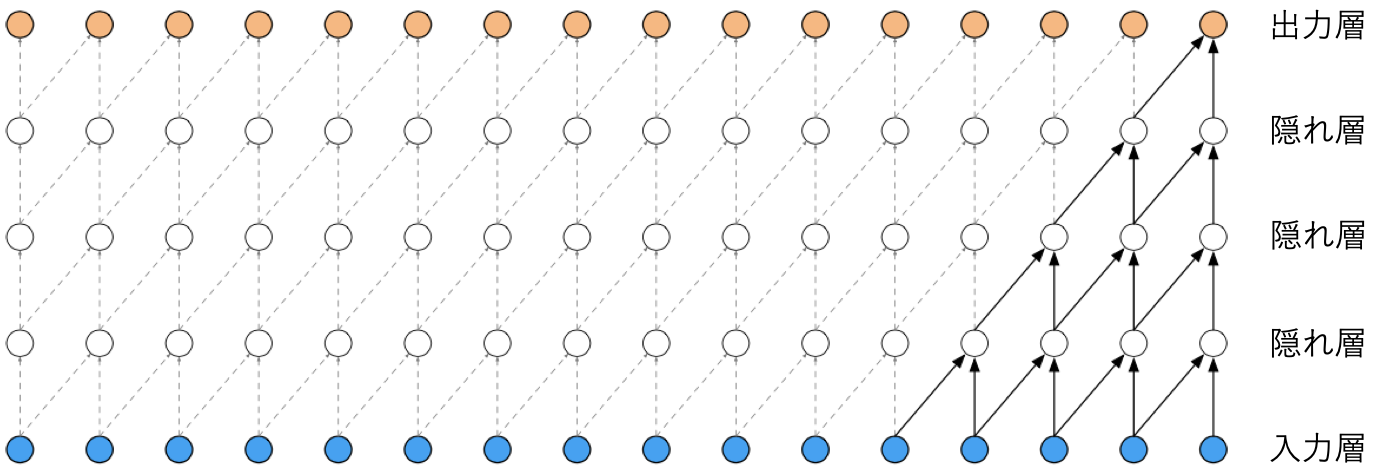
\includegraphics[width=\linewidth]{./figure/ccl.png}
	\caption{因果的畳み込み層}
	\label{fig:ccl}
\end{figure}
